
\section{Overview of Technology}

To build an online real-time multiplayer game, there are two popular approaches known. One approach is \ptoP \emph{lockstep}, is based on \ptoP architecture. In this approach, all clients start in the same initial state and broadcast their actions. The overall performance of the system is dependent on slower clients in the system. Moreover, since the clients use broadcast methods to communicate, the approach has high message complexity.

To achieve better real-time simulation systems switched to a \clientServer model (see Figure~\ref{figure:server-models}(a))~\cite{DOOMfaq}. With this model the state of the game is stored on a server and clients send updates to the server. This works well as latency is determined by the client to server connection. However, this was still too slow for real-time online games, which lead to the introduction of client-side prediction~\cite{bernier2001latency}. Simply put client-side prediction allows the client to simulate its own version of the game (sending the results to the server) but the server can still step in and override the client's game state. This creates complexity in handling server overrides on clients smoothly (not just in code but also in animation and audio). Another reason for this model to gain traction was the ability to handle malicious clients by validating all actions on the server.


This gets very complicated, why have all the infrastructure? Why not just use a peer-to-peer (not lockstep) method? Two reasons, the first is that players could not join a game in progress. Second, the client can (and will) cheat, sending faulty position information to everyone in order to gain an advantage.

It would be nice if we could completely trust clients but we can’t. What if we could trust them a little? If we can trust clients a little we can use them as servers. If we can have a client as server we might be able to reduce latency by choosing the best client to act as the server.

What has not been mentioned in this discussion is fault tolerance. A client/server model has a single point of failure, the server. This can be very bothersome to players of the game that have invested a large amount of time into the game. 

Also having the single server model results in little fault tolerance. Not to mention the company has to construct many expensive servers so the clients can play.

Benefit of this solution:
Having a more fault tolerant system using a distributed server. 
Reducing latency by reducing by picking good servers
All online multiplayer systems are best effort. If we can create a system with the same responsiveness with fault tolerance then it is a success.
% The \ptoP model does handle fault tolerance more gracefully. Having the single server in the \clientServer model results in little fault tolerance.

\subsection{Multiplayer Network Design}

	There are two common networking structures for multiplayer gaming. The first is \ptoP, with the structure each client sends state updated to each other client in the game. A diagram of the \ptoP communication structure is shown in Figure~\ref{figure:p2p-vs-ClientServer}(a).
	The second, and more common, is the \clientServer design. In the \clientServer design each client sends updates to a single server and this server will relay these messages to the other clients playing the game. The communication structure for this design can be seen in Figure~\ref{figure:p2p-vs-ClientServer}(b).
	
\begin{figure}[ht]
	\centering
	\begin{tabular}{c c}
		Peer-to-Peer & Client-Server \\
		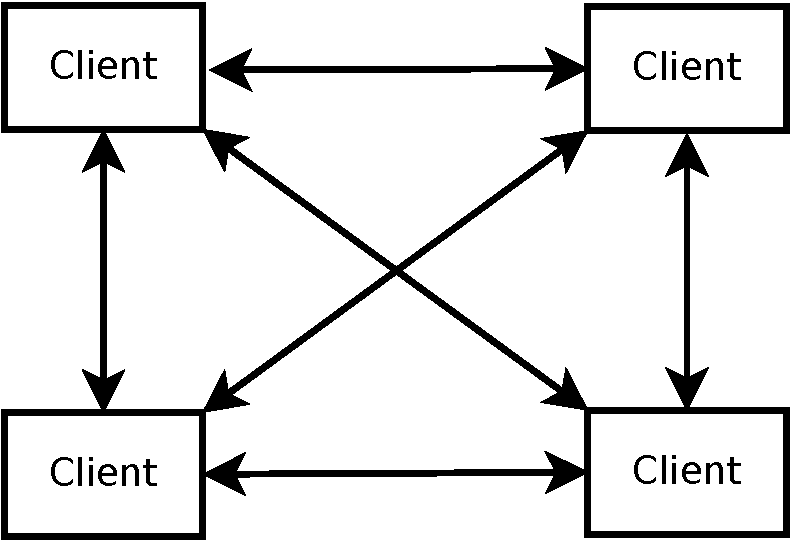
\includegraphics[width=0.48\linewidth]{../images/p2p-model-crop.pdf} &
		%trim=l b r t
		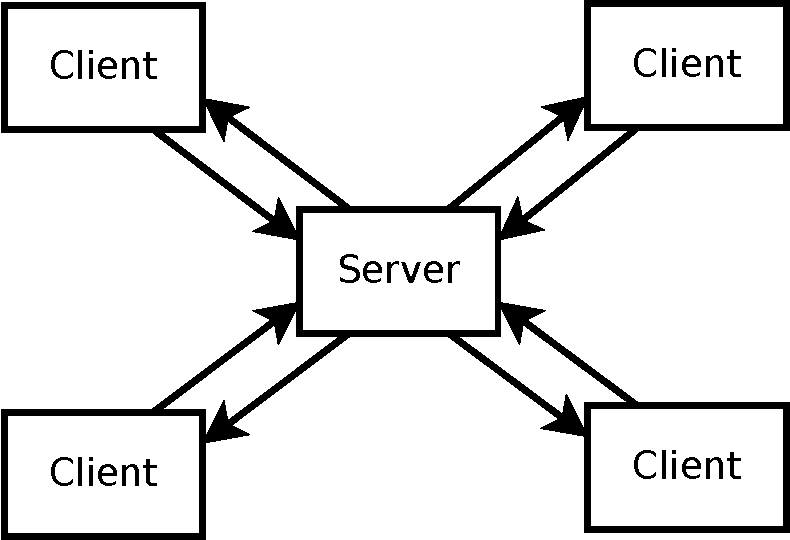
\includegraphics[width=0.48\linewidth]{../images/client-server-model-crop.pdf} \\
		(a) & (b)
	\end{tabular}

	\caption{\label{figure:p2p-vs-ClientServer} Two mutiplayer game networking models. The model on the left (a) is a \ptoP model where every client sends updates directly to ever other client in the game. The second model (b) is a \clientServer model. In this model all of the clients send updates to the server and the server send updates out to the clients.}
	\end{figure}
	
	We choose to base our work off of the \clientServer model for a number of reasons
	\begin{enumerate}
		\item The \clientServer model tends to have less latency
		\item The \clientServer model supports clients joining mid game
		\item The \clientServer model is less susceptible to cheating/malicious clients.
	\end{enumerate}
	
	As in most multiplayer game networking systems asynchronous communication is used. This is necessary to preserve the real-time nature of the game. Packet loss is considered not significant as a new packet with more up-to-date information will be sent soon after the lost packet.
	
